\documentclass{article}
\usepackage{graphicx} 
\usepackage{amsmath}
\usepackage{amssymb}
\usepackage{amsthm}
\usepackage{enumitem}
\usepackage{todonotes}
\usepackage{hyperref}
\usepackage{algorithm,algorithmicx,algpseudocode}

\title{Happy Reconfiguration}
\date{August 2024}

\newtheorem{theorem}{Theorem}[section]
\newtheorem{lemma}[theorem]{Lemma}
\newtheorem{proposition}[theorem]{Proposition}
\newtheorem{observation}[theorem]{Observation}
\newtheorem{cor}[theorem]{Corollary}
\newtheorem{example}[theorem]{Example}
\newtheorem{conjecture}[theorem]{Conjecture}
\newtheorem{rem}[theorem]{Remark}
\newtheorem{definition}[theorem]{Definition}
\newtheorem{corollary}[theorem]{Corollary}
\newtheorem{conj}{Conjecture}[section]


\graphicspath{ {img/} }

\newlist{caseof}{enumerate}{1}
\setlist[caseof,1]{label = Case \arabic*: , wide=0pt, leftmargin=+\labelsep, font=\bfseries, topsep=2pt, itemsep=0pt}%

\author{GADA Lab, University of Manitoba}

\begin{document}

\maketitle

\section{Preliminaries and work so far:}

Let $P$ be a set of $n$ points in convex position, i.e., the convex hull of $P$ is an $n$-sided polygon (or $n$-gon). We will represent the convex hull of $P$ by $CH(P)$.

\begin{definition}[Caterpillar]
	A tree $T$ is called a \emph{caterpillar} if removing its leaves (and their incident edges) produces a path, which is called the \emph{spine} of $T$.
\end{definition}

\begin{definition}[Interior Edge]
	An edge $e$ which is not on the convex hull of a graph drawing in a convex point set $P$ is called an \textbf{interior edge}.
\end{definition}

\begin{definition}[Boundary Edge]
	An edge $e'$ which is not an interior edge is called a \textbf{boundary edge}.
\end{definition}

\begin{lemma}
	\label{lem:two-boundary}
	Every non-crossing spanning tree of a set of points in convex position has at least two boundary edges.
\end{lemma}

\begin{definition}
	An interior edge $e$ cuts $CH(P)$ into two convex regions $R_L(e)$ and $R_R(e)$ on convex point sets $P_L(e)$ and $P_R(e)$, respectively. Given a non-crossing spanning tree $T$ of $P$, the \emph{restriction} of $T$ to $P_L(e)$ (resp., $P_R(e)$) is the subgraph of $T$ induced by the vertices in $P_L(e)$ (resp., $P_R(e)$).
\end{definition}

\begin{observation}
	\label{obs:restriction-is-nst}
	The restriction of $T$ to $P_L(e)$ (resp., $P_R(e)$) is a non-crossing spanning tree of $P_L(e)$ (resp., $P_R(e)$).
\end{observation}

\begin{lemma}
	\label{lem:interior_edge_boundary}
	Given a non-crossing spanning tree $T$ of $P$, any interior edge $e$ cuts the n-gon into exactly two convex polygons who share $e$ as a common edge and each such polygon has at least two boundary edges, one of which is $e$.
\end{lemma}
\begin{proof}[Proof for \ref{lem:interior_edge_boundary}]
	$ $ \\
	Consider the two regions $R_L(e)$ and $R_R(e)$ that $e$ cuts the $CH(P)$ into. By Lemma~\ref{lem:two-boundary}, the restriction of $T$ to $P_L(e)$ has at least two boundary edges, one of which is $e$. Thus, the restriction of $T$ of $P_L(e)$ has at least one boundary edge of $CH(P)$. A similar argument holds for the restriction of $T$ to $P_R(e)$.
\end{proof}


\begin{theorem}[Graph drawing of caterpillar]
	\label{theorem:caterpillar_graph_drawing}
	Given a convex point set $P$, if a graph drawing of a tree $T$ has exactly 2 edges on the convex hull, then $T$ is a caterpillar. In addition, every caterpillar graph can be redrawn such that exactly 2 edges remain on the convex hull.
\end{theorem}
\begin{proof}[Proof for \ref{theorem:caterpillar_graph_drawing}]
	$ $ \\

	\todo{Add proper notation for restriction}
	We will first show that if a graph drawing of a non-crossing spanning tree $T$ has exactly 2 edges on the convex hull, then $T$ is a caterpillar.

	Let the two boundary edges of a graph drawing of a non-crossing spanning tree $T$ be $b_1 = (u_1, v_1)$ and $b_2 = (u_2, v_2)$. We will consider the cases of when $b_1$ and $b_2$ are adjacent and when they are not:

	\begin{caseof}
		\item $b_1$ and $b_2$ are adjacent.\\
		Note that if $b_1$ and $b_2$ are adjacent, then $b_1$ and $b_2$ share a common vertex, say $u_1$.
		If $b_1$ and $b_2$ are adjacent, then the graph drawing of a tree $T$ is a star. We can show this statement holds true by considering an interior edge $e$ that does not contain $u_1$, then we will obtain that both $b_1$ and $b_2$ are only on one of the polygons obtained from when we cut the convex n-gon obtained from the convex point set $P$ using $e$. This would imply that one of the polygons will have 3 boundary edges: $b_1$, $b_2$, and $e$ which is a contradiction from Lemma \ref{lem:interior_edge_boundary} and hence, we obtain a star. Since a star is a caterpillar, we are done.

		\item $b_1$ and $b_2$ are not adjacent.\\
		Let $P = (u_1, v_1, \dots, v_2, u_2)$ be the longest path starting from the endpoint of $b_1$ and ending at the endpoint of $b_2$. Consider the polygons obtained from cutting the n-gon using $P$. We note that each polygon contains exactly two boundary edges (both of which are from the path) and these two edges are adjacent. Then, from Case 1, we see that these edges of the polygons form a star. Since we have stars chained together by a path, once we remove all the leaves of each star, we simply get $P$. Hence, we also get a caterpillar in this case.
	\end{caseof}

	Since we have a caterpillar in both cases, this shows that if a graph drawing of a non-crossing spanning tree $T$ has exactly 2 edges on the convex hull, then $T$ is a caterpillar.
	\\

	Now, we show that every caterpillar graph can be drawn such that exactly 2 edges remain on the convex hull.

	Let $P = \{p_1, p_2, \dots, p_n\}$ be the spine of caterpillar graph. Let $L_i$ be the set of all leaves of the vertex $p_i$.
	Let $B$ be the 4-gon formed by setting $p_1, p_2, p_{n - 1},$ and $p_n$ as its corners, let $CH(B)$ represent the convex hull of $B$.

	\begin{figure}[hbt!]
		\centering
		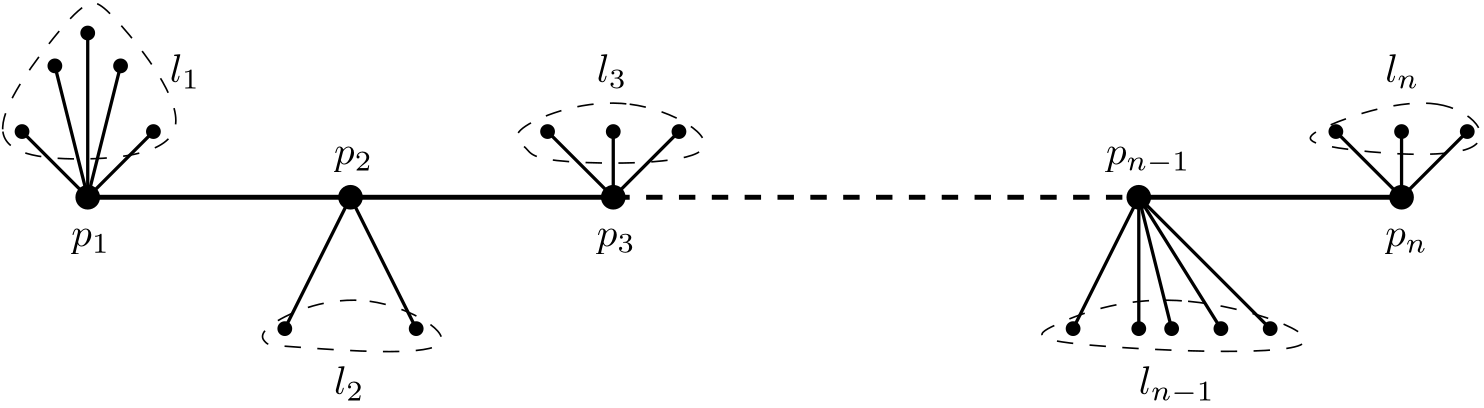
\includegraphics[width=0.8\textwidth]{spine}
		\caption{A caterpillar with spines and leaves labelled.}
	\end{figure}
	\newpage

	Now, align $P$ such that $b_1 = (p_1, p_2)$ and $b_2 = (p_{n - 1}, p_n)$. WLOG, assume that $n$ is even and partition $P$ into two subsets $P_E$ and $P_O$ such that all $p_i$ of $P$ where $i$ is even are in $P_E$ and all $p_j$ of $P$ where $j$ is odd are in $P_O$. In addition, set all the elements of $L_i$ to be in $P_E$ if $i$ is odd and set them to be in $P_O$ if $i$ is even. Note that $p_1$ and $p_{n - 1}$ are both in $P_O$ and $p_2$ and $p_n$ are both in $P_E$. Now, align all the elements of $P_E$ from $P$ such that they lie in the line joining $p_1$ and $p_{n - 1}$ from $CH(B)$. Similarly, align all the elements of $P_O$ from $P$ such that they lie in the line joining $p_2$ and $p_n$ from $CH(B)$. Then, align all the elements of $P_E$ that are leaves such that they fall in between $p_i$ and $p_{i + 1}$ in the line. Do so similarly for $P_O$.


	\begin{figure}[hbt!]
		\centering
		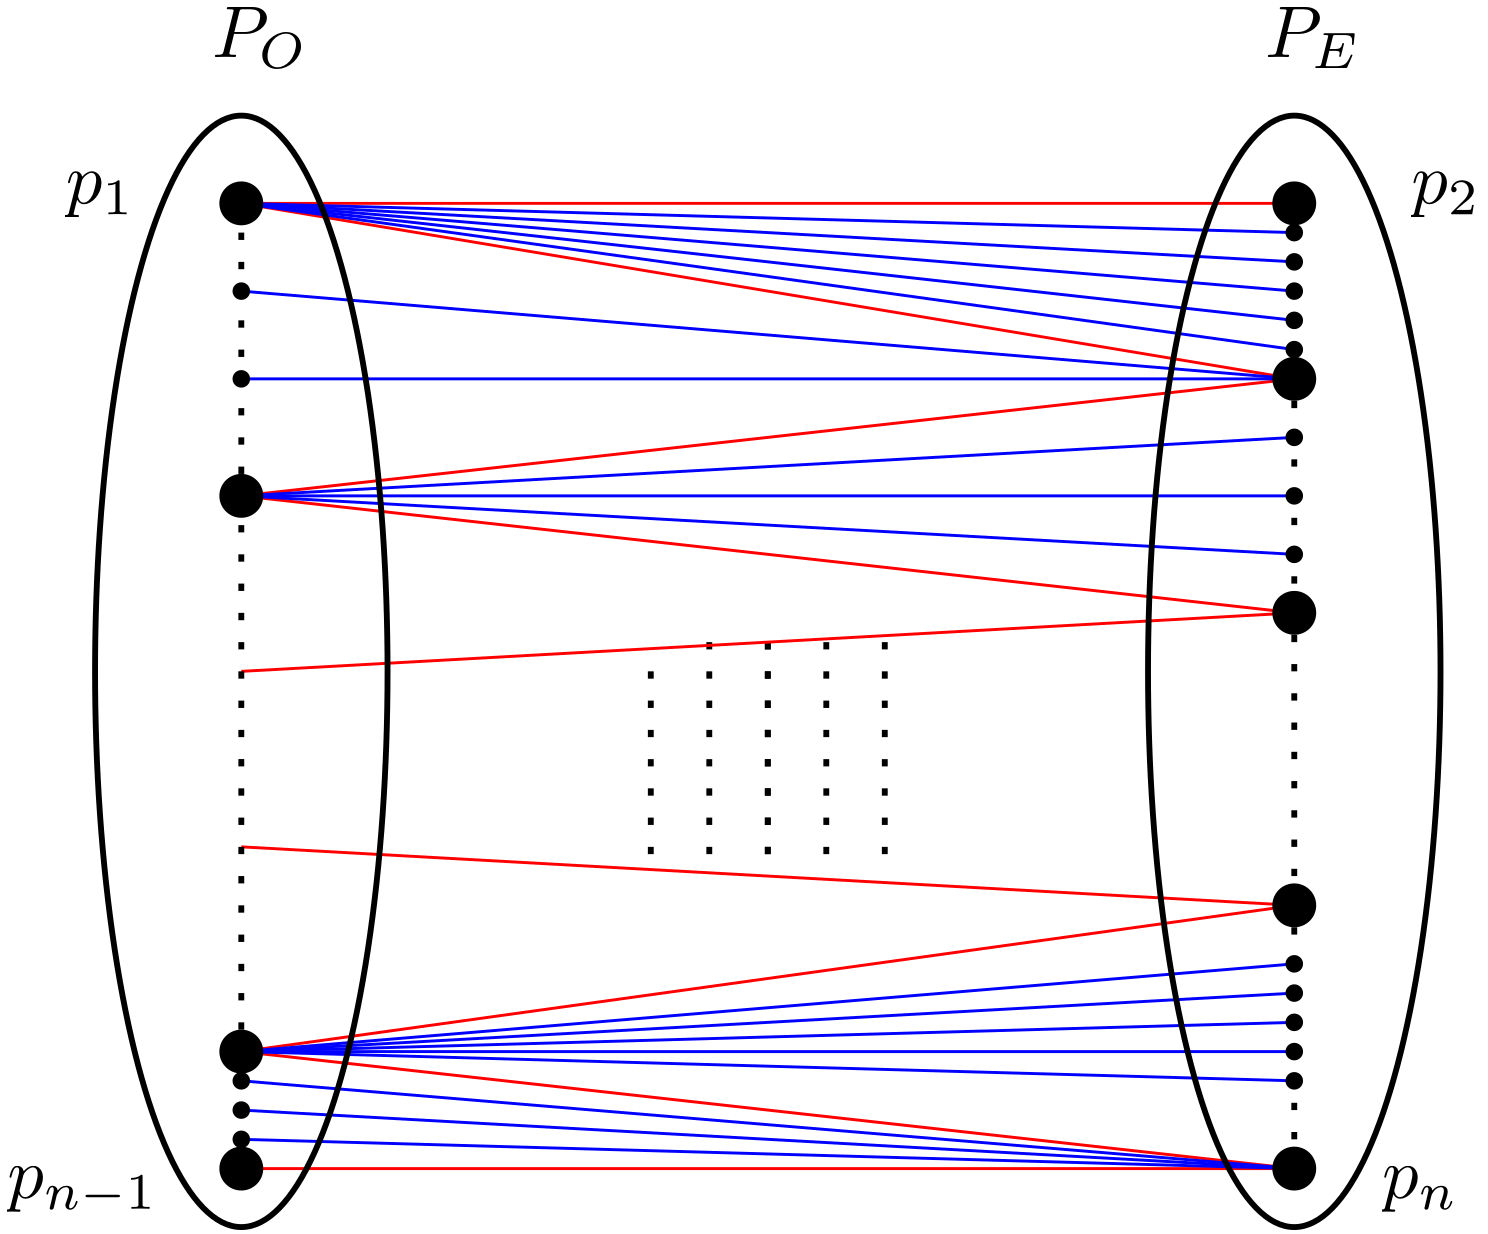
\includegraphics[width=0.5\textwidth]{partitioned_caterpillar}
		\caption{Partitioned caterpillar. The blue edges are the edges with leaves. The red edges are the spine.}
	\end{figure}

	Note that $P_E$ and $P_O$ are disjoint, independent, and non-crossing. Also, observe that there are exactly 2 boundary edges in $B$, namely $b_1$ and $b_2$. And so, we are done.
\end{proof}

\section{Happy Edge Conjecture for Convex Point Sets}

An edge $e$ is \emph{happy} if
$e$ lies in $T_I \cap T_F$.

\begin{lemma} %{\bf[Happy Edge Conjecture for Convex Point Sets]}
	\label{lem:happy-edge}
	For any point set $P$ in convex position and any two non-crossing spanning trees $T_I$ and $T_F$ of $P$, there is a minimum flip sequence from $T_I$ to $T_F$ such that
	no happy edge is flipped during the sequence.
\end{lemma}

Aichholzer et al.~\cite{aichholzer-arxiv-2024}
conjectured that the statement in Lemma~\ref{lem:happy-edge} holds and
proved it for the case of happy edges on the convex hull. We prove that their conjecture indeed holds in the general case.
\begin{proof}
	$ $ \\
	\todo{Add proper notation for restriction}
	We prove by induction on the number of \emph{interior} happy edges, that is, those happy edges that are not on the convex hull.
	For the base case, if there are no interior happy edges, then we use the result of Aichholzer et al.~\cite{aichholzer-arxiv-2024}
	that there is a minimum flip sequence from $T_I$ to $T_F$ without flipping the happy edges.

	Assume now that there are $k$ interior happy edges. Select one such edge $e$ (assume wlog. that it is vertical)
	and observe that no other edge of $T_I$ or $T_F$ crosses $e$.
	Therefore, we can divide the point set $P$ into $P_l$ and $P_r$
	of all the points in $P$ that are to
	the left and to the right of $e$ (including the endpoints of $e$) respectively.
	Similarly, we can divide the tree $T_I$ into subtrees $T_{I,l}$
	and $T_{I,r}$ as well as $T_F$ into non-crossing spanning subtrees $T_{F, l}$ and $T_{F, r}$ embedded onto $P_l$ and $P_r$, respectively (Observation~\ref{obs:restriction-is-nst}).
	Notice that $T_{I,l}$ and $T_{F, l}$ as well as $T_{I, r}$ and $T_{F, r}$ have one less happy edge in their interiors, therefore, by induction
	there is a minimum flip sequence from $T_{I,l}$ to $T_{F, l}$ on $P_l$ and  from $T_{I,r}$ to $T_{F, r}$ on $P_r$ that do not flip their happy edges.
	Observe now that any minimum flip sequence from $T_{I}$ to $T_{F}$ can be partitioned into flips  only on $P_l$ and only on $P_r$
	since no edge can cross $e$. Therefore, we can combine the minimum flip sequence from $T_{I,l}$ to $T_{F, l}$ on $P_l$ and from $T_{I,r}$ to $T_{F, r}$ on $P_r$
	to obtain a minimum flip sequence from $T_{I}$ to $T_{F}$.
\end{proof}

\section{Greedy algorithm [DEPRECATED]}

Rough draft of the algorithm as discussed:

\begin{enumerate}
	\item Select lowest intersecting blue edge and make the number of intersections to the blue edge $0$ by flipping all red edges intersection with it and place it on the boundary. (Idea: While flipping all intersecting red edges, conserve the endpoint closest to the boundary while trying to make it connected).
	\item Now, take the red edge with the most number of intersections and swap it with the blue edge with $0$ intersections. Prioritise the edges placed in the boundary.
	      \begin{itemize}
		      \item If this step creates a cycle then remove the red edges on the boundary and \textit{perfect} flip them into the sub-problem on the region formed by the last removal of the blue edge.
	      \end{itemize}
\end{enumerate}

\section{Algorithm for converting any caterpillar into any other non-crossing spanning tree in $\frac{3n}{2} + c$ steps}


\begin{definition}
	If $R$ is a region, then the length of the path formed on $CH(R)$ is denoted by $\partial(R)$.
\end{definition}

\begin{definition}[Eccentricity of reconfiguration graphs]
	The total distance (i.e, the number of edge flips) from an initial non-crossing spanning tree $T_I$ to a final non-crossing spanning tree $T_F$ is defined to be the \textbf{\textit{eccentricity}} of $T_I$.

	Furthermore, the eccentricity of a graph with $i$ boundary edges is denoted by $e_i$, for $i \in \mathbb{N}$.
\end{definition}

\begin{proposition}[Bound of eccentricity of caterpillar graphs]
	\label{prop:eccentricity-bound-caterpillar}
	The eccentricity of a non-crossing drawing of any caterpillar graph to any other non-crossing spanning tree is bounded by $\frac{3n}{2} \pm c$, for $c \in O(1)$.
\end{proposition}

\begin{proof}
	General idea:

	\begin{enumerate}
		\item Consider the 2 boundary edges of $T_I$, call them $b_1$ and $b_2$. Also, note that we shall color all the edges of $T_I$ as red and color all the edges of $T_F$ as blue.
		\item Notice that $b_1$ and $b_2$ divides $CH(T_I)$ into 2 regions, call them $R_1$ and $R_2$.
		\item Consider the minimum of $\partial(R_1)$ and $\partial(R_2)$. WLOG, say that $\partial(R_1) \leq \partial(R_2)$. Note that $\partial(R_1) \leq \partial(R_2) \leq \dfrac{n}{2}$, where $n$ is the number of vertices. Now, consider $R_1$:


		\item ``Shifting the spine.'' [Iterative argument] (Maximum number of steps taken is at most $\frac{n}{2}$)
		      \begin{itemize}
			      \item Add a red edge on $CH(R_1)$. Since $T_I$ is a tree, adding an edge creates a cycle. To resolve the cycle, delete an edge of that cycle that is not a boundary edge. Note that the resulting tree is still a connected, non-crossing, spanning tree.

			      \item Keep repeating the previous step until $CH(R)$ has its boundary completely covered by red edges.

			      \item The end result will be a caterpillar graph with it's spine on $CH(R_1)$ and all the leaves forming an edge with the spine on $CH(R_1)$.
		      \end{itemize}

		\item We now claim that every edge flip that occurs from now on is a (pseudo) perfect flip. [It is pseudo in the sense that it isn't flipping to the actual $T_F$ but instead converging from both directions to a single tree, say $T_F'$, in n flips.]

		\item ``Shifting'' $T_F$ [Iterative + Inductive argument]
		      \begin{itemize}
			      \item Now, consider $T_F$, we shall apply a similar iterative argument as before.

			      \item Add a blue edge on $CH(R)$. Similarly to the previous case, we will obtain a cycle. To resolve the cycle, delete a non-boundary edge of the cycle. Note that the resulting graph is a connected non-crossing spanning tree.

			      \item Keep repeating the previous step until $CH(R)$ has its boundary completely covered by blue edges.

			      \item Note that every single edge that we flipped only had to be flipped once so each edge only contributes 1 flip.
		      \end{itemize}

		\item Set the cardinal directions as $b_1$ as the `left', $b_2$ as the `right', $R_1$ as the `top', and $R_2$ as the `bottom'.

		      \begin{itemize}
			      \item From \ref{lem:zero-red-crossing-edge}, we know that there exists at least 1 red edge that has 0 crossings. From the algorithm outlined in \ref{lem:zero-red-crossing-edge}, pick the blue edge that is connected to the endpoint of the red edge that has 0 crossings and flip the blue edge to the red edge.
			      \item We now have two smaller subproblems towards the region to the left of the flipped blue edge and towards the right of the flipped blue edge.
			      \item Note that those two sub regions have the same criteria as our main graph and thus we can keep applying \ref{lem:zero-red-crossing-edge} and flipping blue edges to red edges as shown above.
			      \item Also, note that each flip is a perfect flip so each edge only contributes 1 flip.
		      \end{itemize}

		\item Finally, from the above two steps, we know that we can flip the blue tree into the red shifted spine tree in at most $n$ steps. Combining everything, we get that the total number of flips from any red non-crossing spanning caterpillar to any blue non-crossing spanning tree is at most $\frac{n}{2} + n = \frac{3n}{2}$ flips.
	\end{enumerate}
\end{proof}

\begin{lemma}
	After the shifting the spine step, there will always be at least 1 red edge that has 0 crossings.
\end{lemma}
\begin{proof}
	\label{lem:zero-red-crossing-edge}
	All the variables follow from the shifting the spine step.
	Set the cardinal directions as $b_1$ as the `left', $b_2$ as the `right', $R_1$ as the `top', and $R_2$ as the `bottom'.

	\begin{itemize}
		\item Pick the closest vertex from $b_1$ and $R_2$, call it $u_1$.
		\item Note that $u_1 \not\in R_1$. However, from our ``Shifting the spine'' step, we know that it is connected to the spine formed in $R_1$ by an edge, call it $e_1$. Now, follow along from $u_1$ to $e_1$ and note each time there is a crossing from a blue edge to $e_1$. Since we are dealing with at most $\frac{n}{2}$ remaining blue edges, there will be at most $\frac{n}{2}$ crossings which is a finite amount. Now, take the last crossing encountered and follow the blue edge that caused the crossing all the way to the endpoint of the blue edge towards $b_1$.
		\item Repeat the above step until you find a red edge that has $0$ crossings.
		\item Say, for contradiction, that after repeating the above steps we do not find a red edge that has $0$ crossings. This implies that we followed a blue edge to an endpoint in $b_2$. Hover since $b_2$ already had both red and blue edges, this implies that there exists a cycle in the blue tree which is a contradiction.
	\end{itemize}
\end{proof}

\bibliographystyle{plain}
\bibliography{refs}
\end{document}

